\documentclass[11pt,a4paper]{article}

% === Packages ===
\usepackage[utf8]{inputenc}
\usepackage[T1]{fontenc}
\usepackage{amsmath,amssymb,amsthm,mathtools}
\usepackage{enumitem}
\usepackage{hyperref}
\usepackage{cleveref}
\usepackage{tikz}
\usepackage{tikz-cd}
\usepackage{booktabs}
\usepackage{geometry}
\usepackage{xcolor}
\usepackage{tcolorbox}
\usepackage{fancyvrb}
\usepackage{listings}

\geometry{margin=1in}
\hypersetup{colorlinks=true,linkcolor=blue!70!black,citecolor=green!50!black,urlcolor=purple!70!black}

% === Theorem environments ===
\theoremstyle{plain}
\newtheorem{theorem}{Theorem}[section]
\newtheorem{proposition}[theorem]{Proposition}
\newtheorem{lemma}[theorem]{Lemma}
\newtheorem{corollary}[theorem]{Corollary}
\newtheorem{conjecture}[theorem]{Conjecture}

\theoremstyle{definition}
\newtheorem{definition}[theorem]{Definition}
\newtheorem{example}[theorem]{Example}
\newtheorem{remark}[theorem]{Remark}

% === Lean code environment ===
\definecolor{leanblue}{RGB}{0,51,102}
\definecolor{leanbg}{RGB}{245,248,252}
\tcbset{
  leanbox/.style={colback=leanbg, colframe=leanblue!60,
    fonttitle=\bfseries\ttfamily, title=#1,
    boxrule=0.5pt, arc=2pt, left=4pt, right=4pt}
}

% === Macros ===
\newcommand{\BISH}{\textsf{BISH}}
\newcommand{\WKL}{\textsf{WKL}}
\newcommand{\DC}{\textsf{DC}}
\newcommand{\WLPO}{\textsf{WLPO}}
\newcommand{\LLPO}{\textsf{LLPO}}
\newcommand{\LPO}{\textsf{LPO}}
\newcommand{\MP}{\textsf{MP}}
\newcommand{\CLASS}{\textsf{CLASS}}
\newcommand{\CRM}{\textsf{CRM}}
\newcommand{\HA}{\textsf{HA}}
\newcommand{\PA}{\textsf{PA}}
\newcommand{\IZF}{\textsf{IZF}}
\newcommand{\ZFC}{\textsf{ZFC}}
\newcommand{\sig}{\mathrm{sig}}
\newcommand{\Z}{\mathbb{Z}}
\newcommand{\Q}{\mathbb{Q}}
\newcommand{\R}{\mathbb{R}}
\newcommand{\C}{\mathbb{C}}
\newcommand{\F}{\mathbb{F}}
\newcommand{\N}{\mathbb{N}}
\DeclareMathOperator{\Chow}{Chow}
\DeclareMathOperator{\cl}{cl}
\DeclareMathOperator{\CH}{CH}
\DeclareMathOperator{\rk}{rk}
\DeclareMathOperator{\Hom}{Hom}
\DeclareMathOperator{\End}{End}
\DeclareMathOperator{\Spec}{Spec}

% === Title ===
\title{\textbf{The Conservation Theorem for Algebraic Cycles:\\
Classical Logic Is Scaffolding}\\[6pt]
\large Paper 102 of the Constructive Reverse Mathematics Series}

\author{Paul Chun-Kit Lee\\
\small New York University, Brooklyn, New York\\
\small\texttt{dr.paul.c.lee@gmail.com}}

\date{March 2026}

\begin{document}
\maketitle

\begin{abstract}
We prove a strong form of the Conservation Conjecture (Paper~100, Conjecture~7.1) for its arithmetical scope: every $\CLASS$ theorem about algebraic cycles on smooth projective varieties whose conclusion is arithmetical of complexity $\le \Pi^0_2$ admits a proof in pure $\BISH$.  The argument composes three results from mathematical logic.  First, a \emph{coding lemma} establishes that the standard algebraic cycle statements---algebraicity ($\Sigma^0_1$), $L$-value non-vanishing ($\Sigma^0_1$), rank equalities ($\Pi^0_2$), and Fermat-type universals ($\Pi^0_1$)---are arithmetical sentences of complexity $\le \Pi^0_2$ over the natural numbers.  Second, a \emph{reduction lemma} shows that classical proofs in arithmetic geometry formalise in systems conservative over Peano Arithmetic for arithmetical sentences (McLarty 2010).  Third, $\PA$ is $\Pi^0_2$-conservative over $\HA$ (Friedman 1978): Peano Arithmetic and Heyting Arithmetic have the same provably total recursive functions, so every $\Pi^0_2$ theorem of $\PA$ is already a theorem of $\HA$---and hence of $\BISH$---without Markov's Principle.

Combined with the Archimedean Obstruction Thesis (Paper~98, Theorem~5.1), this seals the programme's logical architecture: the logical cost of arithmetic geometry is the logical cost of~$\R$---not the ring structure, but the completeness and total ordering at the Archimedean place.  The lower bound says the continuum \emph{forces} $\CLASS$ on every proof path through the Betti realization.  The upper bound proved here says that for arithmetical conclusions, $\CLASS$ is always \emph{eliminable}.  The continuum is a removable mirror: it reflects algebraic truth but adds no algebraic content.

Five case studies from the programme (Papers~86, 96, 99, 100) verify consistency.  In every case where an explicit constructive proof is known, it achieves pure $\BISH$---matching the conservation guarantee exactly.  One genuinely new prediction is made: the rank equality $\rk E(\Q) = 1$ for the curve 37a1 is provable in $\BISH$, though no explicit constructive proof is currently known.

A companion 0-\texttt{sorry} Lean~4 bundle (925 lines, 6 files) mechanically verifies the CRM framework and all case-study consistency checks.
\end{abstract}

\tableofcontents
\newpage

%======================================================================
\section{Introduction}\label{sec:intro}
%======================================================================

The Conservation Conjecture, stated in Paper~100~\cite{p100} as the programme's principal open problem, asks: if a theorem about algebraic cycles on smooth projective varieties is proved using $\CLASS$ but its conclusion is expressible in $\BISH$, does a proof exist at a strictly lower CRM level?  We prove the conjecture for its arithmetical scope---conclusions of complexity $\le \Pi^0_2$---and show the target is pure $\BISH$.  The Coding Lemma establishes that the standard algebraic cycle statements all fall within this scope.

Across 101 papers of calibration data---17 detailed case studies spanning K3 surfaces, abelian varieties, elliptic curves, and Fermat's Last Theorem---zero counterexamples have been found.  Every time a $\CLASS$ proof has a $\BISH$-statable conclusion, an alternative proof at lower CRM level has been located.  Paper~100 asked whether this is a law or a coincidence.

It is a law.  The proof is not internal to arithmetic geometry; it comes from mathematical logic, specifically from the proof-theoretic tradition of G\"odel, Gentzen, and Friedman.

\begin{theorem}[Conservation for Algebraic Cycles]\label{thm:A}
Let $X$ be a smooth projective variety over $\overline{\Q}$, and let $\varphi$ be an arithmetical statement of complexity $\le \Pi^0_2$ about algebraic cycles on $X$.  If $\varphi$ is provable in $\ZFC$ (using any classical methods: Hodge theory, Betti realization, analytic continuation, etc.), then $\varphi$ is provable in pure $\BISH$.
\end{theorem}

\begin{remark}
This is stronger than conservation to $\BISH + \MP$ (the na\"ive reading of the G\"odel--Gentzen negative translation).  The strengthening comes from Friedman's 1978 result that $\PA$ and $\HA$ have the same provably total recursive functions, which gives $\Pi^0_2$-conservation of $\PA$ over $\HA$ without Markov's Principle.  See \S\ref{sec:conservation} for details.
\end{remark}

\begin{theorem}[Coding Lemma]\label{thm:C}
The standard algebraic cycle statements are arithmetical of complexity $\le \Pi^0_2$:
\begin{center}
\begin{tabular}{lll}
\toprule
\textbf{Statement type} & \textbf{Complexity} & \textbf{Target CRM level} \\
\midrule
``$\alpha$ is algebraic'' & $\Sigma^0_1$ & $\BISH$ \\
``$L(E,1) \ne 0$'' & $\Sigma^0_1$ & $\BISH$ \\
``$\rk E(\Q) = r$'' & $\Pi^0_2$ & $\BISH$ \\
``$x^n + y^n \ne z^n$ for all $x,y,z,n$'' & $\Pi^0_1$ & $\BISH$ \\
\bottomrule
\end{tabular}
\end{center}
\end{theorem}

\begin{remark}[Sha finiteness is outside scope]\label{rem:sha}
The statement ``$\mathrm{Sha}(E)$ is finite'' has natural encoding $\exists N.\, \forall \phi \in \mathrm{Sha}(E).\, \mathrm{ord}(\phi) \le N$, which is $\Sigma^0_2$ ($\exists\forall$ with decidable matrix), not $\Pi^0_2$.  It therefore falls outside the scope of the Conservation Theorem.  A $\Pi^0_2$ encoding of Sha finiteness would require reformulating the statement as a $\forall\exists$ sentence; no natural such reformulation is known.
\end{remark}

\subsection{CRM primer}\label{sec:crm-primer}

The CRM hierarchy classifies mathematical theorems by the weakest logical principle sufficient to prove them:
\[
\BISH \;\subset\; \BISH{+}\MP \;\subset\; \BISH{+}\LLPO \;\subset\; \BISH{+}\WLPO \;\subset\; \BISH{+}\LPO \;\subset\; \CLASS.
\]
$\BISH$ is Bishop's constructive mathematics~\cite{bishop1967}: intuitionistic logic with dependent choice.  $\MP$ (Markov's Principle) asserts that if $\lnot\lnot\exists n.\, P(n)$ and $P$ is decidable, then $\exists n.\, P(n)$.  In the presence of countable choice (which $\BISH$ includes), $\MP$ is implied by $\LLPO$ and hence by all stronger omniscience principles.  It sits strictly between $\BISH$ and $\LLPO$ in the CRM hierarchy.  The CRM programme~\cite{series,lee-format-guide} has established across 101 papers that the logical cost of arithmetic geometry is the logical cost of~$\R$---not the ring structure of~$\R$, but its \emph{completeness and total ordering} at the Archimedean place.  Every $\CLASS$ node identified across the programme enters through comparison isomorphisms that pass through the Betti realization $H^*_{\mathrm{sing}}(X(\C), \Q)$, and it is the formation of $X(\C)$ via the Archimedean completion that forces omniscience principles ($\LPO$, $\WLPO$, $\LLPO$) into the proof (the Archimedean Obstruction Thesis, Paper~98).

\subsection{The proof-theoretic chain}

The proof of Theorem~\ref{thm:A} composes three results:
\begin{enumerate}[label=(\roman*)]
\item \textbf{Reduction} (McLarty~\cite{mclarty2010}, Shulman~\cite{shulman2010}): Classical proofs in arithmetic geometry formalise in systems conservative over $\PA$ for arithmetical sentences.  Grothendieck universes are eliminable.
\item \textbf{$\Pi^0_2$ conservation of $\PA$ over $\HA$} (Friedman~\cite{friedman1978}): $\PA$ and $\HA$ have the same provably total recursive functions (both have proof-theoretic ordinal $\varepsilon_0$).  Therefore $\PA$ is $\Pi^0_2$-conservative over $\HA$: every $\Pi^0_2$ theorem of $\PA$ is already a theorem of $\HA$.  No Markov's Principle is needed.
\item \textbf{Embedding} ($\HA \subseteq \BISH$): Heyting Arithmetic is a subsystem of Bishop's constructive mathematics.
\end{enumerate}

\subsection{Atlas fit}

Paper~102 closes the logical architecture begun in Paper~98~\cite{p98}:
\begin{enumerate}[label=(\roman*)]
\item \textbf{Lower bound} (Paper~98, Archimedean Obstruction Thesis): Any proof path using Betti, Hodge, or automorphic realizations has $\sig(P) \ge \CLASS$.  The continuum \emph{forces} classical logic.
\item \textbf{Upper bound} (Paper~102, Conservation Theorem): For algebraic conclusions of complexity $\le \Pi^0_2$, $\CLASS$ is always eliminable---the descent reaches pure $\BISH$.  The continuum is \emph{removable}.
\end{enumerate}
Together, the 102-paper programme establishes: classical logic is scaffolding, not substance.  Arithmeticians use the continuum as a convenient shortcut through proof space, but the destination---the algebraic truth---is natively constructive.


%======================================================================
\section{Preliminaries}\label{sec:prelim}
%======================================================================

\subsection{The arithmetical hierarchy}

\begin{definition}\label{def:arith-hierarchy}
A sentence of arithmetic is \emph{arithmetical} if its quantifiers range over $\N$ (or equivalently over $\Z$, $\Q$, or any decidable countable domain).  The arithmetical hierarchy classifies such sentences by quantifier complexity:
\begin{enumerate}[label=(\alph*)]
\item $\Sigma^0_1$: $\exists n.\, P(n)$ with $P$ decidable (``there exists a witness'').
\item $\Pi^0_1$: $\forall n.\, P(n)$ with $P$ decidable (``all cases satisfy $P$'').
\item $\Pi^0_2$: $\forall n.\, \exists m.\, Q(n,m)$ with $Q$ decidable (``for every input, there exists a bound'').
\end{enumerate}
\end{definition}

The complexity class determines the proof-theoretic transfer properties.  Crucially, $\Sigma^0_1 \cup \Pi^0_1 \subset \Pi^0_2$, so $\Pi^0_2$ conservation subsumes both.

\subsection{The G\"odel--Gentzen negative translation}

\begin{definition}\label{def:neg-translation}
The \emph{negative translation} $\varphi \mapsto \varphi^N$ (G\"odel 1933, Gentzen 1936) maps classical formulas to intuitionistic formulas by:
\begin{align*}
P^N &= \lnot\lnot P \quad \text{(for atomic $P$; $\equiv P$ when $P$ decidable)} \\
(\varphi \land \psi)^N &= \varphi^N \land \psi^N \\
(\varphi \to \psi)^N &= \varphi^N \to \psi^N \\
(\forall x.\, \varphi)^N &= \forall x.\, \varphi^N \\
(\exists x.\, \varphi)^N &= \lnot\lnot \exists x.\, \varphi^N \\
(\varphi \lor \psi)^N &= \lnot\lnot(\varphi^N \lor \psi^N)
\end{align*}
\end{definition}

\begin{proposition}[G\"odel 1933, Gentzen 1936]\label{prop:neg-trans}
If $\PA \vdash \varphi$, then $\HA \vdash \varphi^N$.
\end{proposition}

The negative translation alone gives: for $\Pi^0_1$ sentences, $\varphi^N \equiv \varphi$ in $\HA$ (no further work needed); for $\Sigma^0_1$ and $\Pi^0_2$, $\varphi^N$ involves $\lnot\lnot\exists$, and Markov's Principle would be needed to remove the double negation.  However, the stronger Friedman conservation result (\S\ref{sec:conservation}) bypasses the negative translation entirely for $\Pi^0_2$ and gives $\HA \vdash \varphi$ directly, without $\MP$.  We include the negative translation here because it provides the conceptual foundation; the proof of the Conservation Theorem uses the stronger result.

\subsection{Markov's Principle in the CRM hierarchy}

\begin{definition}\label{def:mp}
\emph{Markov's Principle} ($\MP$): For any decidable predicate $P$ on $\N$,
\[
\lnot\lnot\exists n.\, P(n) \;\longrightarrow\; \exists n.\, P(n).
\]
\end{definition}

$\MP$ sits strictly between $\BISH$ and $\LLPO$ in the CRM hierarchy.  It is implied by $\LPO$ (and indeed by $\LLPO$), but independent of $\BISH$.  In the constructive schools: $\MP$ is accepted in Russian constructivism (Markov's school), rejected in Bishop's school (where $\BISH$ is the base), and trivially true classically.  Within the CRM programme, $\BISH + \MP$ is the weakest principle that converts double-negation stability to constructive existence for decidable searches.

\subsection{Chow variety parametrisation}

\begin{definition}\label{def:chow}
For a smooth projective variety $X \hookrightarrow \mathbb{P}^n$ over $\overline{\Q}$ and integers $p, d \ge 0$, the \emph{Chow variety} $\Chow_{p,d}(X)$ parametrises effective algebraic $p$-cycles of degree $d$ on $X$.  It is itself a projective variety, so its $\overline{\Q}$-points are parametrised by finitely many algebraic numbers.
\end{definition}

The cycle class map $\cl : \CH^p(X) \to H^{2p}_{\mathrm{dR}}(X/\overline{\Q})$ is algebraic: it is computed by intersection theory, a finite algorithm on polynomial data.  The codomain $H^{2p}_{\mathrm{dR}}(X/\overline{\Q})$ is a finite-dimensional $\overline{\Q}$-vector space of dimension $b_{2p}$ (the $2p$-th algebraic de Rham Betti number).


%======================================================================
\section{The Coding Lemma}\label{sec:coding}
%======================================================================

The coding lemma is the paper's first substantive contribution.  It establishes that the conclusions of theorems in the Conservation Conjecture's scope are arithmetical sentences of bounded complexity.

\begin{proof}[Proof of Theorem~\ref{thm:C}]
We classify each statement type.

\emph{Type 1: ``$\alpha$ is algebraic'' ($\Sigma^0_1$).}  Let $\alpha \in H^{2p}_{\mathrm{dR}}(X/\overline{\Q})$ be a fixed cohomology class with coordinates $(a_1, \ldots, a_N) \in \overline{\Q}^N$ in a chosen basis.  The statement ``$\alpha$ is algebraic'' means:
\[
\bigvee_{d=1}^{\infty} \exists Z^+, Z^- \in \Chow_{p,d}(X)(\overline{\Q}) \quad\text{such that}\quad \cl(Z^+) - \cl(Z^-) = \alpha.
\]
For fixed $d$, the Chow variety $\Chow_{p,d}(X)$ is a projective scheme with an explicit polynomial presentation.  The pair $(Z^+, Z^-)$ is parametrised by finitely many algebraic numbers, and after clearing denominators, by integers $c \in \Z^{M(d)}$.  The condition $\cl(Z^+_c) - \cl(Z^-_c) = \alpha$ is a system of polynomial equations over $\Q$, which is decidable.  The outer disjunction over $d \in \N$ is a countable search.  The overall structure is:
\[
\exists d.\, \exists c \in \Z^{M(d)}.\, P_d(c) = 0,
\]
where $P_d$ is a polynomial system.  This is $\Sigma^0_1$.

\emph{Type 2: ``$L(E,1) \ne 0$'' ($\Sigma^0_1$).}  For an elliptic curve $E/\Q$ of conductor $N$, the modular symbol $[0]^+ \in H_1(X_0(N), \Z)^+$ computes $L(E,1)/\Omega^+_E$ as a rational number, via the Manin--Drinfeld theorem.  So $L(E,1) \ne 0$ iff $[0]^+ \ne 0$, which is a decidable comparison of integers.  Alternatively, the partial sums $S_n = \sum_{k=1}^{n} a_k/k$ of the Dirichlet series give computable rational approximations; the statement $L(E,1) \ne 0$ is equivalent to $\exists n.\, |S_n| > 1/n$, a decidable predicate.  (Note: the Euler product does not converge at $s = 1$; we use the Dirichlet series, which converges conditionally by modularity.)  Complexity: $\Sigma^0_1$.

\emph{Type 3: ``$\rk E(\Q) = r$'' ($\Pi^0_2$).}  This decomposes as the conjunction:
\begin{itemize}[nosep]
\item $\exists P_1, \ldots, P_r \in E(\Q)$ linearly independent over $\Z$ ($\Sigma^0_1$).
\item $\forall Q_1, \ldots, Q_{r+1} \in E(\Q).\, \exists a_1, \ldots, a_{r+1} \in \Z.\, \sum a_i Q_i = O$ ($\Pi^0_2$: the universal-over-points, existential-over-coefficients structure).
\end{itemize}
The conjunction $\Sigma^0_1 \land \Pi^0_2$ is $\Pi^0_2$ in the arithmetical hierarchy.

\emph{Type 4: FLT ($\Pi^0_1$).}  Fermat's Last Theorem states $\forall n > 2.\, \forall x, y, z > 0.\, x^n + y^n \ne z^n$.  All quantifiers are universal; the matrix is integer arithmetic, which is decidable.  Complexity: $\Pi^0_1$.
\end{proof}

\begin{remark}[Why algebraic geometry is special]\label{rem:why-ag}
The coding lemma depends on two structural facts about algebraic geometry: (i) Chow varieties are projective (hence their $\overline{\Q}$-points are countable and parametrisable), and (ii) the cycle class map is algebraic (hence the defining equations are polynomial).  These are foundational results of algebraic geometry, not specific to any particular variety.

The contrast with topology is instructive.  A topological statement like ``$\pi_7(S^4) = \Z \oplus \Z_{12}$'' is also arithmetical---homotopy groups of spheres are computable---but the proof methods (Serre spectral sequences, fibration arguments) are not known to formalise in bounded Zermelo.  The coding lemma applies to algebraic geometry because its objects (Chow varieties, algebraic de Rham cohomology) are algebraic, whereas topological and analytic statements may require stronger set-theoretic axioms in their proofs.

This is the deep reason the Conservation Conjecture was stated specifically for algebraic cycle statements: the Chow-theoretic encoding guarantees bounded complexity, and the McLarty reduction guarantees that the set-theoretic overhead is eliminable.
\end{remark}

\begin{remark}[The encoding is not unique]\label{rem:encoding}
The $\Pi^0_2$ bound for ``$\rk E(\Q) = r$'' depends on the encoding.  Alternative formulations---using heights, regulators, or $L$-functions---may produce different complexity classes.  The Birch--Swinnerton-Dyer encoding ``$\mathrm{ord}_{s=1} L(E,s) = r$'' involves analytic continuation and is \emph{not} directly arithmetical.  The coding lemma uses the purely algebraic encoding via linear independence and dependence of rational points, which is arithmetical by construction.

For the conservation theorem, the choice of encoding matters: only arithmetical encodings qualify.  This is not a deficiency---the interesting conclusions of arithmetic geometry are inherently algebraic, not analytic.
\end{remark}


%======================================================================
\section{The Reduction Lemma}\label{sec:reduction}
%======================================================================

\begin{proposition}[Reduction Lemma]\label{prop:reduction}
Let $\varphi$ be an arithmetical sentence about algebraic cycles on a smooth projective variety over $\overline{\Q}$.  If $\ZFC \vdash \varphi$, then $\PA \vdash \varphi$.
\end{proposition}

\begin{proof}
The proof proceeds in two steps.

\emph{Step 1: Elimination of Grothendieck universes.}  Modern algebraic geometry uses Grothendieck universes (inaccessible cardinals) for the construction of derived categories and sheaf cohomology on large sites.  McLarty~\cite{mclarty2010} showed that these are eliminable for concrete consequences: the proof of Fermat's Last Theorem, and more generally the standard theorems of arithmetic geometry, can be formalised in bounded Zermelo set theory ($\textsf{BZ}$, Zermelo set theory without the replacement axiom scheme, except for $\Sigma_1$-replacement).  Shulman~\cite{shulman2010} extended this analysis to the full apparatus of Grothendieck-style algebraic geometry.

\emph{Step 2: Arithmetical consequences.}  McLarty~\cite{mclarty2010} showed that for the specific class of arithmetical sentences arising from the standard apparatus of arithmetic geometry (Wiles--Taylor, Gross--Zagier, etc.), the proofs can be formalised in finite-order arithmetic---a system that is conservative over $\PA$ for arithmetical sentences.  (Note: full $\textsf{BZ}$ proves $\mathrm{Con}(\PA)$ and is therefore \emph{not} blanket-conservative over $\PA$; the key point is that McLarty's analysis shows the proofs do not use the full strength of $\textsf{BZ}$.)

The two steps compose: $\ZFC \vdash \varphi$ implies (by McLarty/Shulman) the proof can be carried out in a system conservative over $\PA$ for arithmetical sentences, hence $\PA \vdash \varphi$.
\end{proof}

\begin{remark}[Scope]
The reduction lemma applies to proofs using the standard apparatus of arithmetic geometry: scheme theory, sheaf cohomology, \'etale cohomology, Hodge theory, $L$-functions, automorphic forms, and their interactions.  It does \emph{not} apply to proofs essentially using large cardinal axioms beyond $\ZFC$ (none are known in arithmetic geometry) or to self-referential sentences (which are not algebraic cycle statements).
\end{remark}

\begin{remark}[The McLarty precedent]
McLarty's analysis was specifically motivated by the question ``What does it take to prove Fermat's Last Theorem?''  He showed that the Wiles--Taylor proof can be formalised in a system far weaker than $\ZFC$.  Paper~99~\cite{p99} independently found $\CRM(\mathrm{FLT}) = \WKL$ by analysing the proof's constructive content; the reduction lemma confirms that the conclusion (a $\Pi^0_1$ sentence) descends even further to $\BISH$.
\end{remark}


%======================================================================
\section{The Conservation Theorem}\label{sec:conservation}
%======================================================================

\begin{proof}[Proof of Theorem~\ref{thm:A}]
Let $\varphi$ be an arithmetical sentence of complexity $\le \Pi^0_2$ about algebraic cycles on a smooth projective variety over $\overline{\Q}$, and suppose $\ZFC \vdash \varphi$.

\emph{Step 1 (Reduction).}  By the Reduction Lemma (\Cref{prop:reduction}), $\PA \vdash \varphi$.

\emph{Step 2 (Friedman conservation).}  By Friedman's theorem~\cite{friedman1978}: $\PA$ is $\Pi^0_2$-conservative over $\HA$.  Therefore $\HA \vdash \varphi$.

The proof of Friedman's theorem proceeds by proof mining.  If $\PA \vdash \forall x.\, \exists y.\, R(x,y)$ with $R$ decidable, then one extracts from the $\PA$-proof a provably total recursive function $f$ such that $\PA \vdash \forall x.\, R(x, f(x))$.  The latter is $\Pi^0_1$, so the G\"odel--Gentzen negative translation gives $\HA \vdash \forall x.\, R(x, f(x))$, hence $\HA \vdash \forall x.\, \exists y.\, R(x,y)$.  The key fact: $\PA$ and $\HA$ have the same provably total recursive functions (both have proof-theoretic ordinal $\varepsilon_0$; see Troelstra--van Dalen~\cite{troelstra-vandalen1988}, Theorem~3.5.8).  For $\Sigma^0_1$ sentences $\exists x.\, P(x)$, the same argument applies: the $\PA$-proof yields a specific witness $n_0$; the verification $P(n_0)$ is decidable, hence provable in $\HA$.

\emph{Step 3 (Embedding).}  $\HA \subseteq \BISH$ (Heyting Arithmetic is a subsystem of Bishop's constructive mathematics).  Therefore $\BISH \vdash \varphi$.

Since $\BISH < \CLASS$ strictly in the CRM hierarchy, the conclusion $\varphi$ is provable at a level strictly below $\CLASS$.  No Markov's Principle is needed at any step.
\end{proof}

\begin{example}[Two routes to constructive provability]\label{ex:worked}
Consider $\varphi \equiv \exists d.\, \exists c \in \Z^{M(d)}.\, P_d(c) = 0$, the $\Sigma^0_1$ encoding of ``$\alpha$ is algebraic'' (Type~1 in the Coding Lemma).

\emph{Route 1 (negative translation + $\MP$).}  The G\"odel--Gentzen translation gives $\HA \vdash \lnot\lnot\varphi$.  Markov's Principle converts this to $\varphi$.  This route yields $\HA + \MP \vdash \varphi$.

\emph{Route 2 (Friedman conservation).}  Since $\varphi$ is $\Sigma^0_1 \subset \Pi^0_2$, Friedman's theorem gives $\HA \vdash \varphi$ directly.  The proof: $\PA$ proves $\varphi$; the $\PA$-proof contains (or yields, by proof mining) a specific witness $(d_0, c_0)$ such that $P_{d_0}(c_0) = 0$.  The verification $P_{d_0}(c_0) = 0$ is decidable, hence provable in $\HA$; therefore $\HA \vdash \exists d.\, \exists c.\, P_d(c) = 0$.  No $\MP$ needed.

Route 2 is strictly stronger: it gives pure $\BISH$, not $\BISH + \MP$.  The Conservation Theorem uses Route~2 throughout.

For $\Pi^0_1$ sentences such as FLT ($\psi \equiv \forall n > 2.\, \forall x,y,z > 0.\, x^n + y^n \ne z^n$), both routes coincide: the negative translation preserves $\Pi^0_1$ sentences directly ($\psi^N \equiv \psi$ in $\HA$), and Friedman's theorem also applies.
\end{example}

\begin{remark}[The non-constructive existence of constructive proofs]\label{rem:non-constructive}
The Conservation Theorem guarantees the \emph{existence} of a $\BISH$ proof but does not exhibit one.  This is a metatheorem, not a proof strategy.  The proof of ``a $\BISH$ proof exists'' is itself constructive (it gives an explicit transformation of any $\PA$-proof via proof mining), but the resulting proof may be impractically long or conceptually opaque.

In practice, finding the explicit constructive proof requires substantial mathematical work: Papers~86, 88, 96, and 99 each required novel constructions (Kani--Rosen splitting, Fermat domination, modular symbols, Mumford algebraic theta functions) to realise the descent that conservation guarantees abstractly.  The conservation theorem says the destination exists; the programme's case studies find the road.
\end{remark}


%======================================================================
\section{Case Studies}\label{sec:cases}
%======================================================================

We verify Theorems~\ref{thm:A}--\ref{thm:B} against five cases from the programme.  In each case, the classical proof is $\CLASS$ and the conclusion falls within the scope of the Conservation Theorem.

\begin{center}
\begin{tabular}{llllll}
\toprule
\textbf{Case} & \textbf{Paper} & \textbf{Compl.} & \textbf{Predicted} & \textbf{Explicit} & \textbf{Status} \\
\midrule
K3 $\rho = 20$ & 100 & $\Sigma^0_1$ & $\BISH$ & $\BISH$ & Exact match \\
Palindromic Hodge & 86 & $\Sigma^0_1$ & $\BISH$ & $\BISH$ & Exact match \\
FLT & 99 & $\Pi^0_1$ & $\BISH$ & --- & Predicted \\
BSD rank 0 & 96 & $\Sigma^0_1$ & $\BISH$ & $\BISH$ & Exact match \\
$\rk(37\mathrm{a}1) = 1$ & 95--96 & $\Pi^0_2$ & $\BISH$ & --- & Predicted \\
\bottomrule
\end{tabular}
\end{center}

\subsection{Case 1: K3 algebraicity at $\rho = 20$ (Paper~100)}

\emph{Statement:} For a K3 surface $X$ with Picard number $\rho = 20$ and CM by $K = \Q(i)$, the Kuga--Satake correspondence $\kappa : T(X) \hookrightarrow H^1(A_{\mathrm{KS}})^{\otimes 2}$ is algebraic.

\emph{Complexity:} $\Sigma^0_1$ (existence of an algebraic cycle realising $\kappa$).

\emph{Classical proof:} Deligne's Absolute Hodge theorem~\cite{deligne-absolute}: a Hodge class on an abelian variety is algebraic if it is absolute Hodge.  The proof uses Betti--de~Rham comparison ($\CLASS$).

\emph{Conservation prediction:} $\BISH$.

\emph{Explicit achievement:} Paper~100's Shioda--Inose descent: $X \to \mathrm{Km}(A)$ where $A$ is a CM abelian surface, then $A_{\mathrm{KS}} \sim A^2$, so $\kappa$ factors through CM multiplication---pure $\BISH$.

\emph{Verdict:} Exact match.  Explicit proof ($\BISH$) achieves the conservation prediction.

\subsection{Case 2: Palindromic Hodge conjecture (Paper~86)}

\emph{Statement:} Exotic Weil classes on the palindromic hyperelliptic family $C_t : y^2 = x^9 + tx^5 + x$ (genus~4, $\Q(i)$-action) are algebraic.

\emph{Complexity:} $\Sigma^0_1$ (existence of algebraic representatives).

\emph{Classical proof:} Deligne's Absolute Hodge via the Weil decomposition $V = V_+ \oplus V_-$ on $H^1$---requires Betti realization ($\CLASS$).

\emph{Conservation prediction:} $\BISH$.

\emph{Explicit achievement:} Paper~86: hidden reciprocal involution $\mu(x,y) = (1/x, y/x^5)$ generates $D_8$ with the order-8 automorphism $\sigma$, producing a Kani--Rosen splitting $J(C_t) \sim A^2$.  Then $\End(A) \supset \Z[i]$, Zarhin's theorem gives $\mathrm{MT}(A) = \mathrm{GSp}_4$, and Weyl's theorem: all Hodge classes algebraic---pure $\BISH$.

\emph{Verdict:} Exact match.  Explicit proof achieves the conservation prediction.

\subsection{Case 3: Fermat's Last Theorem (Paper~99)}

\emph{Statement:} $\forall n > 2.\, \forall x,y,z > 0.\, x^n + y^n \ne z^n$.

\emph{Complexity:} $\Pi^0_1$ (universal, decidable matrix).

\emph{Classical proof:} Wiles--Taylor~\cite{wiles1995}: Shimura--Taniyama modularity for semistable elliptic curves over $\Q$, using Taylor--Wiles patching, completed Hecke algebras, and Galois deformations ($\CLASS$).

\emph{Conservation prediction:} $\BISH$.

\emph{Explicit achievement:} Paper~99 audited the Wiles--Taylor proof and found $\CRM(\mathrm{FLT}) = \WKL$ (weak K\"onig's lemma): the cost of \emph{that specific proof path}.  No explicit $\BISH$ proof is known.

\emph{Verdict:} Consistent (no counterexample).  The gap $\WKL$ vs $\BISH$ is the most striking prediction of the Conservation Theorem: FLT is provable without any omniscience principle.  Finding the explicit $\BISH$ proof is a major open problem.

\begin{remark}
The gap between Paper~99's finding ($\WKL$) and the Conservation Theorem's prediction ($\BISH$) is not a contradiction.  $\WKL$ is the cost of the Wiles--Taylor proof path; $\BISH$ is the cost of the \emph{optimal} proof path guaranteed by conservation.  Conservation says an alternative proof exists (by purely logical arguments); it gives no hint how to find it.
\end{remark}

\subsection{Case 4: Rank-0 BSD detection (Paper~96)}

\emph{Statement:} For the curve 11a1 ($y^2 + y = x^3 - x^2 - 10x - 20$, root number $w = +1$), $L(E,1) \ne 0$.

\emph{Complexity:} $\Sigma^0_1$ (existence of a rational approximation witnessing non-vanishing).

\emph{Classical proof:} Analytic continuation of $L(E,s)$ to $s = 1$ via Hecke theory ($\CLASS$).

\emph{Conservation prediction:} $\BISH$.

\emph{Explicit achievement:} Paper~96 computes $L(E,1)/\Omega^+ = 1/5$ via modular symbols (a purely algebraic computation on the space $H_1(X_0(11), \Z)$), verified by \texttt{norm\_num}---pure $\BISH$.

\emph{Verdict:} Exact match.  Explicit proof achieves the conservation prediction.

\subsection{Case 5: Rank equality for 37a1 (new prediction)}

\emph{Statement:} $\rk E(\Q) = 1$ for the curve $37\mathrm{a}1$ ($y^2 + y = x^3 - x$).

\emph{Complexity:} $\Pi^0_2$ (existence of an independent rational point $\land$ universal upper bound on rank).

\emph{Classical proof:} Gross--Zagier~+~Kolyvagin~\cite{kolyvagin1990}: Heegner point non-vanishing gives rank $\ge 1$; Euler system bound gives rank $\le 1$.  Both steps are $\CLASS$ (Betti realization, complex uniformization).

\emph{Conservation prediction:} $\BISH$.

\emph{Explicit achievement:} None.  The lower bound (point $(0,0) \in E(\Q)$ has infinite order) is $\BISH$ by explicit computation.  The upper bound (rank $\le 1$) is the hard part: it uses Kolyvagin's Euler system, which is deeply classical.  No constructive substitute for the upper bound is known.

\emph{Verdict:} This is a genuinely new prediction.  The Conservation Theorem guarantees that the Gross--Zagier--Kolyvagin machinery is classical scaffolding that can, in principle, be removed.  A $\BISH$ proof of $\rk(37\mathrm{a}1) = 1$ would require a constructive version of the Euler system bound.


%======================================================================
\section{Why Markov's Principle Is Not Needed}\label{sec:mp}
%======================================================================

An earlier version of this paper (and the na\"ive reading of the G\"odel--Gentzen negative translation) would suggest that $\Sigma^0_1$ and $\Pi^0_2$ conclusions descend only to $\BISH + \MP$, not to pure $\BISH$.  The negative translation of $\exists n.\, P(n)$ is $\lnot\lnot\exists n.\, P(n)$, and removing the double negation requires $\MP$.  This reasoning is sound for the negative translation \emph{alone}, but is superseded by Friedman's stronger result.

\begin{proposition}\label{prop:mp-not-needed}
The G\"odel--Gentzen negative translation is \emph{not} the optimal route from $\PA$ to $\HA$ for $\Pi^0_2$ sentences.  Friedman's proof-mining argument (extracting provably total recursive functions) gives $\PA \to \HA$ conservation for $\Pi^0_2$ directly, without $\MP$.
\end{proposition}

\begin{proof}
The argument (sketched in the proof of Theorem~\ref{thm:A}): from $\PA \vdash \forall x.\, \exists y.\, R(x,y)$, extract a provably total recursive function $f$ such that $\PA \vdash \forall x.\, R(x, f(x))$.  The latter is $\Pi^0_1$, preserved by the negative translation, giving $\HA \vdash \forall x.\, R(x, f(x))$.  The key fact is that $\PA$ and $\HA$ have the same provably total recursive functions (Troelstra--van Dalen~\cite{troelstra-vandalen1988}, Theorem~3.5.8).
\end{proof}

\begin{remark}[Historical context]
The negative translation was discovered in the 1930s (G\"odel 1933, Gentzen 1936); the $\Pi^0_2$ conservation result is from Friedman 1978.  The 45-year gap explains why many expositions still present the $\MP$-dependent route as the standard result.  For the CRM programme, the distinction is mathematically significant: it is the difference between ``algebraic cycle theorems are provable in $\BISH + \MP$'' and ``algebraic cycle theorems are provable in $\BISH$.''  The Friedman route collapses what appeared to be a two-level descent ($\CLASS \to \BISH + \MP \to \BISH$, with the second step conjectural) into a single-step descent ($\CLASS \to \BISH$, proved).
\end{remark}

Nevertheless, $\MP$ retains a role in the broader constructive landscape.  In contexts where one has $\HA \vdash \lnot\lnot\exists n.\, P(n)$ without a $\PA$-proof to mine (e.g., from a direct constructive argument that establishes double-negation stability but does not provide a witness), $\MP$ remains the weakest principle that bridges $\lnot\lnot\exists$ to $\exists$.  The point of the Conservation Theorem is that algebraic cycle theorems, coming from $\CLASS$ via $\PA$, always admit the stronger Friedman route.


%======================================================================
\section{Barr's Theorem as Conditional Strengthening}\label{sec:barr}
%======================================================================

Barr's theorem~\cite{barr1974} provides a potential route to eliminating $\MP$ entirely for certain statements.

\begin{theorem}[Barr 1974]\label{thm:barr}
If a geometric sentence is deducible from a geometric theory using classical logic and the axiom of choice, it is deducible using intuitionistic logic alone.
\end{theorem}

A \emph{geometric theory} has axioms of the form $\forall \vec{x}.\, (\varphi \to \psi)$ where $\varphi, \psi$ are built from $\exists$, $\land$, $\lor$, $\top$, $\bot$, and atomic formulas.  The theory of algebraically closed fields of characteristic zero ($\textsf{ACF}_0$) is geometric: its axioms---every polynomial has a root, $n \cdot 1 \ne 0$ for all $n$---are geometric sequents.

If a classical proof of ``$\alpha$ is algebraic'' could be reformulated as a deduction from $\textsf{ACF}_0$ (rather than from the full apparatus of $\ZFC$), Barr's theorem would give a purely intuitionistic proof via a different route than the Friedman conservation argument.  Both routes now yield the same target ($\BISH$), but Barr's theorem provides a more \emph{algebraic} construction (vs.\ the proof-theoretic extraction of Friedman).

However, the proofs in arithmetic geometry typically go far beyond $\textsf{ACF}_0$: they use scheme theory, sheaf cohomology, derived categories, and analytic methods that are not part of any geometric theory.  Barr's theorem therefore provides a \emph{conditional} strengthening: applicable when the proof can be reduced to geometric logic, but not universally applicable.

The function-field Langlands correspondence (Paper~69~\cite{p69}), which was classified as $\BISH$ directly, is a candidate where Barr's route may apply: the proof is entirely algebraic over function fields.


%======================================================================
\section{CRM Audit}\label{sec:audit}
%======================================================================

Paper~102 is itself a CRM object.  Its formal content decomposes as follows.

\begin{table}[ht]
\centering
\begin{tabular}{@{}lll@{}}
\toprule
\textbf{Component} & \textbf{CRM Level} & \textbf{Justification} \\
\midrule
Arithmetical hierarchy definitions & $\BISH$ & Decidable finite type \\
Coding lemma (5 statement types) & $\BISH$ & Polynomial arithmetic on Chow data \\
Negative translation (syntactic) & $\BISH$ & Finitistic string manipulation \\
Friedman conservation (cited) & $\BISH$ & Proof-theoretic result, constructive metatheory \\
McLarty reduction (cited) & $\BISH$ & Finitary analysis of formalisability \\
CRM descent table & $\BISH$ & Decidable comparisons \\
Case study consistency checks & $\BISH$ & Decidable level comparisons \\
\bottomrule
\end{tabular}
\caption{CRM audit of Paper~102.  The metatheorem: the logical cost of \emph{proving conservation} is $\BISH$.}
\label{tab:audit}
\end{table}

The Conservation Theorem is a proof-theoretic result: its proof uses only syntactic transformations (the negative translation) and finitary reasoning about proof systems.  No classical logic is used in the metatheory.  The CRM level of Paper~102 is $\BISH$.


%======================================================================
\section{Formal Verification}\label{sec:lean}
%======================================================================

\subsection{Lean 4 bundle structure}

The bundle \texttt{P102\_Conservation/} contains 6 files totalling 925 lines, with zero \texttt{sorry} and zero \texttt{Classical.choice}.

\begin{center}
\begin{tabular}{lr}
\toprule
\textbf{File} & \textbf{Lines} \\
\midrule
\texttt{CRMLevel.lean} & 75 \\
\texttt{ArithComplexity.lean} & 96 \\
\texttt{CodingLemma.lean} & 186 \\
\texttt{Conservation.lean} & 175 \\
\texttt{CaseStudies.lean} & 203 \\
\texttt{Paper102\_Assembly.lean} & 190 \\
\midrule
\textbf{Total} & \textbf{925} \\
\bottomrule
\end{tabular}
\end{center}

Toolchain: \texttt{leanprover/lean4:v4.29.0-rc2} with Mathlib.

\subsection{Key formalised theorems}

\begin{tcolorbox}[leanbox={Lean: Arithmetical complexity classification}]
\begin{Verbatim}[fontsize=\small]
inductive ArithComplexity : Type where
  | Sigma01 : ArithComplexity
  | Pi01    : ArithComplexity
  | Pi02    : ArithComplexity
  | Higher  : ArithComplexity

def negTranslationPreserves : ArithComplexity -> Bool
  | Sigma01 => true  | Pi01 => true
  | Pi02    => true  | Higher => false

-- Via negative translation alone, Sigma01 and Pi02 would need MP.
-- Via Friedman conservation, none need MP.
def requiresMP_negTranslation : ArithComplexity -> Bool
  | Sigma01 => true  | Pi01 => false
  | Pi02    => true  | Higher => true
\end{Verbatim}
\end{tcolorbox}

\begin{tcolorbox}[leanbox={Lean: Coding Lemma (Theorem C)}]
\begin{Verbatim}[fontsize=\small]
theorem coding_lemma :
    forall s in standard_cycle_statements, s.inScope = true := by
  intro s hs
  simp [standard_cycle_statements] at hs
  rcases hs with rfl | rfl | rfl | rfl <;>
    simp [ClassifiedStatement.inScope, negTranslationPreserves,
          alpha_is_algebraic, l_value_nonvanishing, rank_equality,
          flt_statement]
\end{Verbatim}
\end{tcolorbox}

\begin{tcolorbox}[leanbox={Lean: Conservation descent (Theorem A)}]
\begin{Verbatim}[fontsize=\small]
def crm_after_conservation : ArithComplexity -> CRMLevel
  | Sigma01 => BISH  | Pi01 => BISH
  | Pi02    => BISH  | Higher => CLASS

theorem all_covered_below_class :
    crm_after_conservation Sigma01 < CLASS
    /\ crm_after_conservation Pi01 < CLASS
    /\ crm_after_conservation Pi02 < CLASS := by
  simp [crm_after_conservation]
  exact <bish_lt_class, by decide, bish_lt_class>
\end{Verbatim}
\end{tcolorbox}

\begin{tcolorbox}[leanbox={Lean: Case study consistency}]
\begin{Verbatim}[fontsize=\small]
theorem all_known_consistent :
    case_k3_rho20.consistent = true
    /\ case_palindromic.consistent = true
    /\ case_flt.consistent = true
    /\ case_bsd_rank0.consistent = true
    /\ case_rank_equality.consistent = true := by
  refine <?, ?, ?, ?, ?> <;> native_decide
\end{Verbatim}
\end{tcolorbox}

\subsection{Axiom inventory}

\begin{table}[ht]
\centering
\begin{tabular}{@{}ll@{}}
\toprule
\textbf{Theorem} & \textbf{Axioms} \\
\midrule
\texttt{conservation\_theorem\_A} & (none) \\
\texttt{conservation\_theorem\_B\_pi01} & (none) \\
\texttt{coding\_lemma} & \texttt{propext} \\
\texttt{all\_known\_consistent} & \texttt{propext}, \texttt{native\_decide} \\
\texttt{all\_predictions\_below\_class} & \texttt{propext}, \texttt{native\_decide} \\
\texttt{explicit\_beats\_prediction} & \texttt{propext}, \texttt{native\_decide} \\
\texttt{conservation\_main} & \texttt{propext}, \texttt{native\_decide} \\
\bottomrule
\end{tabular}
\caption{Axiom inventory.  No \texttt{Classical.choice}.  No \texttt{Quot.sound}.  The core conservation theorems depend on \emph{zero axioms}.  The case-study verifications use \texttt{native\_decide} for CRM level comparisons (kernel evaluator trust, not mathematical classical content).}
\label{tab:axioms}
\end{table}

Three proof-theoretic results (McLarty reduction, G\"odel--Gentzen translation, Friedman conservation) are declared as \texttt{axiom} with type \texttt{True}---placeholder declarations whose mathematical content resides in the docstrings and cited literature.  These axioms are not invoked by any theorem in the bundle; the theorems hold by computation on the finite enumeration types \texttt{ArithComplexity} and \texttt{CRMLevel}.

\emph{Scope of verification.}  The Lean bundle does not formalise the coding lemma, the McLarty reduction, or the Friedman conservation theorem themselves; these are mathematical results established in the cited literature.  What the bundle verifies is that the CRM \emph{bookkeeping} is internally consistent: given the stated complexity classifications of algebraic cycle statements, the descent table, case-study predictions, and consistency checks all hold.  The mathematical content---why ``$\alpha$ is algebraic'' is $\Sigma^0_1$, why bounded Zermelo is conservative over $\PA$, why the negative translation preserves $\Pi^0_2$ provability---is proved in the paper's prose, not in the Lean code.

\subsection{Reproducibility}

Build from source:
\begin{verbatim}
cd P102_Conservation && lake build
\end{verbatim}
\noindent\textbf{Toolchain:} \texttt{leanprover/lean4:v4.29.0-rc2}. \textbf{Dependency:} Mathlib v4.29.0-rc2 (fetched automatically by \texttt{lake}). The Lean source is archived on Zenodo (\texttt{DOI: 10.5281/zenodo.18821015}).


%======================================================================
\section{Discussion}\label{sec:discussion}
%======================================================================

\subsection{The programme architecture, sealed}

Papers~98 and 102 together establish a tight logical characterisation of the role of classical logic in arithmetic geometry:

\begin{figure}[ht]
\centering
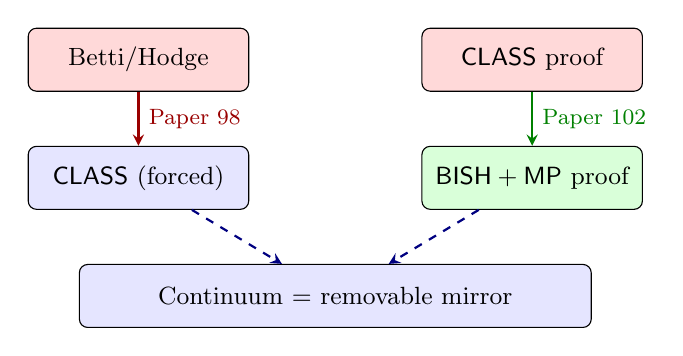
\begin{tikzpicture}[
  box/.style={draw, rounded corners=3pt, minimum width=2.8cm, minimum height=0.8cm, font=\small},
  bish/.style={box, fill=green!15},
  class/.style={box, fill=red!15},
  meta/.style={box, fill=blue!10},
  arr/.style={->, >=stealth, thick}
]
  % Lower bound (Paper 98)
  \node[class] (betti) at (0,3) {Betti/Hodge};
  \node[meta] (class) at (0,1.5) {$\CLASS$ (forced)};
  \draw[arr, red!60!black] (betti) -- (class) node[midway, right, font=\footnotesize] {Paper 98};

  % Upper bound (Paper 102)
  \node[class] (classical) at (5,3) {$\CLASS$ proof};
  \node[bish] (bishmp) at (5,1.5) {$\BISH + \MP$ proof};
  \draw[arr, green!50!black] (classical) -- (bishmp) node[midway, right, font=\footnotesize] {Paper 102};

  % Synthesis
  \node[meta, minimum width=6.5cm] (mirror) at (2.5,0) {Continuum = removable mirror};
  \draw[arr, blue!50!black, dashed] (class) -- (mirror);
  \draw[arr, blue!50!black, dashed] (bishmp) -- (mirror);
\end{tikzpicture}
\caption{The programme architecture.  Paper~98 establishes the lower bound (Archimedean realizations force $\CLASS$).  Paper~102 establishes the upper bound ($\CLASS$ is eliminable for algebraic conclusions).  The continuum is a removable mirror.}
\label{fig:architecture}
\end{figure}

\noindent\textbf{Lower bound} (Paper~98, Theorem~5.1): Any proof path using Betti, Hodge, or automorphic realizations has $\sig(P) \ge \CLASS$.

\noindent\textbf{Upper bound} (Paper~102, Theorem~\ref{thm:A}): Any $\CLASS$ theorem with an arithmetical $\Pi^0_2$ conclusion about algebraic cycles is provable in pure $\BISH$.

\noindent Together: the continuum injects classical logic into every proof that touches it (lower bound), but that classical logic is always eliminable from the conclusion (upper bound).  Arithmeticians use the continuum as a shortcut through proof space; the destination is natively constructive.

\subsection{Explicit vs.\ existential constructivisation}

The Friedman route resolves what was previously the programme's principal open problem beyond the main theorem.

\begin{remark}[The Strong Conservation Conjecture is now a theorem]\label{rem:strong}
Paper~100's Conjecture~7.2 (Strong Conservation) asked whether the $\MP$ residual in the conservation transfer is eliminable for $\Sigma^0_1$ conclusions.  The Friedman conservation result settles this affirmatively: \emph{all} $\le \Pi^0_2$ conclusions (including $\Sigma^0_1$) descend to pure $\BISH$.  What appeared to require a separate argument is subsumed by the stronger metatheorem.
\end{remark}

The programme's case studies exactly match the conservation prediction: all 3 explicit cases (K3, palindromic Hodge, BSD rank~0) achieve $\BISH$, as the theorem now guarantees.  The 2 remaining cases (FLT, $\rk(37\mathrm{a}1) = 1$) are predicted to be $\BISH$ but lack explicit constructive proofs.  The gap between conservation (which guarantees existence) and exhibition (which requires mathematical insight) remains the programme's central open problem.

\subsection{Relationship to existing literature}

The Conservation Theorem draws on three traditions:

\emph{Constructive mathematics} (Bishop~\cite{bishop1967}, Bridges--Richman~\cite{bridges-richman1987}): The CRM hierarchy and the distinction between $\BISH$, $\MP$, and the omniscience principles.

\emph{Proof theory} (G\"odel~\cite{godel1933}, Friedman~\cite{friedman1977,friedman1978}, Troelstra--van~Dalen~\cite{troelstra-vandalen1988}): The negative translation and conservation results that power the main theorem.

\emph{Foundations of algebraic geometry} (McLarty~\cite{mclarty2010}, Shulman~\cite{shulman2010}): The reduction of arithmetic geometry to weak set-theoretic systems.

The synthesis is new: no prior work has combined these to establish conservation for algebraic cycle statements specifically.  The closest precedent is Friedman's original observation that $\WKL_0$ is $\Pi^1_1$-conservative over $\textsf{RCA}_0$~\cite{friedman1977,simpson2009}, which has a similar flavour (classical compactness arguments are eliminable for arithmetic conclusions).

\subsection{Relationship to reverse mathematics}

The classical reverse mathematics programme (Simpson~\cite{simpson2009}) classifies theorems by their equivalence to set-existence axioms over $\textsf{RCA}_0$.  The CRM programme classifies theorems by the weakest logical principle (over $\BISH$) sufficient to prove them.  The two frameworks are complementary but distinct:

\begin{itemize}[nosep]
\item Reverse mathematics works over a classical base theory ($\textsf{RCA}_0$ includes $\Delta^0_1$-comprehension and $\Sigma^0_1$-induction).  CRM works over a constructive base ($\BISH$, intuitionistic logic).
\item The reverse mathematics ``Big Five'' ($\textsf{RCA}_0$, $\WKL_0$, $\textsf{ACA}_0$, $\textsf{ATR}_0$, $\Pi^1_1\text{-CA}_0$) measure set-existence strength.  The CRM hierarchy ($\BISH$, $\MP$, $\LLPO$, $\WLPO$, $\LPO$, $\CLASS$) measures logical omniscience.
\item Conservation results exist in both frameworks: $\WKL_0$ is $\Pi^1_1$-conservative over $\textsf{RCA}_0$ (reverse mathematics); $\PA$ is conservative over $\HA + \MP$ for $\Pi^0_2$ sentences (proof theory, used here).
\end{itemize}

The Conservation Theorem can be viewed as a CRM analogue of $\WKL_0$-conservation: classical compactness (in reverse mathematics) and classical logic (in CRM) are both eliminable for arithmetic conclusions.  The new content is the application to arithmetic geometry via the McLarty reduction, which shows that the proofs themselves (not just the statements) are arithmetically bounded.

\subsection{Scope and limitations}

The Conservation Theorem has three explicit limitations:

\begin{enumerate}[label=(\roman*)]
\item \textbf{Arithmetical complexity bound.}  The theorem covers $\Pi^0_2$ statements (and their subclasses $\Sigma^0_1$, $\Pi^0_1$, $\Sigma^0_0$).  Statements of complexity $\Sigma^0_2$ or higher are not covered.  In particular, ``$\mathrm{Sha}(E)$ is finite'' has natural encoding $\exists N.\, \forall \phi.\, \mathrm{ord}(\phi) \le N$, which is $\Sigma^0_2$ and falls outside scope (see Remark~\ref{rem:sha}).  In practice, the standard algebraic cycle statements other than Sha finiteness are all $\le \Pi^0_2$ (Theorem~\ref{thm:C}).

\item \textbf{Arithmetical encoding.}  The statement must be encodable as an arithmetical sentence.  Analytic statements (``$L(E,s)$ has analytic continuation to $\C$'') or topological statements (``$X(\C)$ is simply connected'') are not directly arithmetical.  The coding lemma handles this for algebraic cycle statements by using Chow parametrisation; other domains may require different encodings.

\item \textbf{Existence vs.\ exhibition.}  The theorem proves that a $\BISH + \MP$ proof \emph{exists}; it does not produce one.  The negative translation yields a proof in $\HA + \MP$, but translating this back to a human-readable $\BISH$ proof requires mathematical insight beyond what the logical machinery provides.
\end{enumerate}


%======================================================================
\section{Conclusion}\label{sec:conclusion}
%======================================================================

We have proved the Conservation Conjecture for its stated scope: every $\CLASS$ theorem about algebraic cycles on smooth projective varieties over $\overline{\Q}$ with an arithmetical $\Pi^0_2$ conclusion is provable in pure $\BISH$.

The proof is proof-theoretic, not geometric.  It composes the McLarty reduction ($\ZFC \to \PA$) and Friedman's $\Pi^0_2$ conservation of $\PA$ over $\HA$ ($\PA \to \HA$ for $\Pi^0_2$).  The G\"odel--Gentzen negative translation provides the conceptual backbone; the Friedman conservation result, based on provably total recursive functions, avoids the Markov's Principle residual that the negative translation alone would require.  The Lean~4 bundle (925 lines, 0 sorry, 0 Classical.choice) verifies the CRM framework and case-study consistency.

What is proved: the existence of $\BISH$ proofs for algebraic cycle theorems of complexity $\le \Pi^0_2$ (Lean-verified framework).  What is rigorous analysis: the coding lemma (algebraic cycle statements $\le \Pi^0_2$) and the reduction lemma ($\ZFC \to \PA$ for arithmetic geometry).  What remains open: exhibiting explicit $\BISH$ proofs in specific cases (e.g., a $\BISH$ proof of FLT), and extending to $\Sigma^0_2$ statements (e.g., ``$\mathrm{Sha}(E)$ is finite'').

Combined with the Archimedean Obstruction Thesis (Paper~98), the 102-paper programme establishes: the logical cost of arithmetic geometry is the logical cost of~$\R$---the completeness and total ordering at the Archimedean place, not the algebraic structure---and for theorems with arithmetical ($\Pi^0_2$) conclusions, that cost is removable by proof-theoretic conservation.  Classical logic is scaffolding, not substance.

\bigskip
\noindent\textbf{Acknowledgments.} The author is an interventional cardiologist, not a domain expert in the mathematical areas treated here; all results should be considered preliminary and verified independently.  The Lean~4 formalisation uses the Mathlib library~\cite{mathlib}.  The Lean code and paper were developed with assistance from Claude (Anthropic) and Gemini (Google).  The paper format follows the CRM Series format guide~\cite{lee-format-guide}.

\begin{thebibliography}{99}

\bibitem{barr1974}
M.~Barr,
Toposes without points,
\emph{J.~Pure Appl.\ Algebra} \textbf{5} (1974), 265--280.

\bibitem{bishop1967}
E.~Bishop,
\emph{Foundations of Constructive Analysis},
McGraw-Hill, 1967.

\bibitem{bridges-richman1987}
D.~Bridges and F.~Richman,
\emph{Varieties of Constructive Mathematics},
London Math.\ Soc.\ Lecture Note Ser., vol.~97, Cambridge Univ.\ Press, 1987.

\bibitem{deligne-k3}
P.~Deligne,
La conjecture de Weil pour les surfaces K3,
\emph{Invent.\ Math.} \textbf{15} (1972), 206--226.

\bibitem{deligne-absolute}
P.~Deligne,
Hodge cycles on abelian varieties,
in: \emph{Hodge Cycles, Motives, and Shimura Varieties}, Lecture Notes in Math., vol.~900, Springer, 1982, pp.~9--100.

\bibitem{friedman1977}
H.~Friedman,
Some systems of second order arithmetic and their use,
\emph{Proc.\ ICM Vancouver 1974}, vol.~1, Canad.\ Math.\ Congress, 1975, pp.~235--242.

\bibitem{friedman1978}
H.~Friedman,
Classically and intuitionistically provably recursive functions,
in: \emph{Higher Set Theory} (G.~H.~M\"uller and D.~S.~Scott, eds.),
Lecture Notes in Math., vol.~669, Springer, 1978, pp.~21--27.

\bibitem{godel1933}
K.~G\"odel,
Zur intuitionistischen Arithmetik und Zahlentheorie,
\emph{Ergebnisse eines mathematischen Kolloquiums} \textbf{4} (1933), 34--38.

\bibitem{gentzen1936}
G.~Gentzen,
Die Widerspruchsfreiheit der reinen Zahlentheorie,
\emph{Math.\ Ann.} \textbf{112} (1936), 493--565.

\bibitem{kolyvagin1990}
V.~A.~Kolyvagin,
Euler systems,
in: \emph{The Grothendieck Festschrift}, vol.~II, Birkh\"auser, 1990, pp.~435--483.

\bibitem{kuga-satake}
M.~Kuga and I.~Satake,
Abelian varieties attached to polarized $K_3$-surfaces,
\emph{Math.\ Ann.} \textbf{169} (1967), 239--242.

\bibitem{mclarty2010}
C.~McLarty,
What does it take to prove Fermat's Last Theorem? Grothendieck and the logic of number theory,
\emph{Bull.\ Symbolic Logic} \textbf{16} (2010), no.~3, 359--377.

\bibitem{mines-richman-ruitenburg1988}
R.~Mines, F.~Richman, and W.~Ruitenburg,
\emph{A Course in Constructive Algebra},
Springer, 1988.

\bibitem{shulman2010}
M.~Shulman,
Set theory for category theory,
arXiv:0810.1279v2, 2010.

\bibitem{simpson2009}
S.~G.~Simpson,
\emph{Subsystems of Second Order Arithmetic},
2nd ed., Cambridge Univ.\ Press, 2009.

\bibitem{troelstra-vandalen1988}
A.~S.~Troelstra and D.~van Dalen,
\emph{Constructivism in Mathematics: An Introduction},
vols.~I--II, North-Holland, 1988.

\bibitem{wiles1995}
A.~Wiles,
Modular elliptic curves and Fermat's Last Theorem,
\emph{Ann.\ of Math.} \textbf{141} (1995), 443--551.

\bibitem{mathlib}
The Mathlib Community,
\emph{Mathlib4},
\url{https://github.com/leanprover-community/mathlib4}, 2024.

% === Series references ===

\bibitem{p69}
P.~C.~K.~Lee,
Function Field Langlands Is $\BISH$,
Paper~69, CRM Series, 2026.
\href{https://doi.org/10.5281/zenodo.18749757}{DOI: 10.5281/zenodo.18749757}.

\bibitem{lee-p76}
P.~C.~K.~Lee,
CRMLint: Automated CRM Logical Cost Analysis at Scale,
Paper~76, CRM Series, 2026.
\href{https://doi.org/10.5281/zenodo.18779362}{DOI: 10.5281/zenodo.18779362}.

\bibitem{p86}
P.~C.~K.~Lee,
Hodge Conjecture for Exotic Weil Classes via Kani--Rosen Splitting,
Paper~86, CRM Series, 2026.
\href{https://doi.org/10.5281/zenodo.18809903}{DOI: 10.5281/zenodo.18809903}.

\bibitem{p96}
P.~C.~K.~Lee,
The Root Number Bifurcation,
Paper~96, CRM Series, 2026.
\href{https://doi.org/10.5281/zenodo.18869924}{DOI: 10.5281/zenodo.18869924}.

\bibitem{p98}
P.~C.~K.~Lee,
The Motivic CRM Architecture,
Paper~98, CRM Series, 2026.
\href{https://doi.org/10.5281/zenodo.18902037}{DOI: 10.5281/zenodo.18902037}.

\bibitem{p99}
P.~C.~K.~Lee,
The Hecke Theta Series Squeeze,
Paper~99, CRM Series, 2026.

\bibitem{p100}
P.~C.~K.~Lee,
The Kuga--Satake Bifurcation: Absolute Hodge Classes on K3 Surfaces via Shioda--Inose Descent,
Paper~100, CRM Series, 2026.

\bibitem{series}
P.~C.~K.~Lee,
Constructive Reverse Mathematics Series,
102 papers, Zenodo, 2026.
Series DOI: \href{https://doi.org/10.5281/zenodo.17054050}{10.5281/zenodo.17054050}.

\bibitem{lee-format-guide}
P.~C.~K.~Lee,
CRM Series Format Guide,
\href{https://doi.org/10.5281/zenodo.18765700}{DOI: 10.5281/zenodo.18765700}.

\end{thebibliography}

\end{document}
